\documentclass[conference]{IEEEtran}
\IEEEoverridecommandlockouts
\usepackage{cite}
\usepackage{amsmath,amssymb,amsfonts}
\usepackage{graphicx}
\usepackage{textcomp}
\usepackage{xcolor}
\usepackage{hyperref}
\usepackage{float}
\usepackage{subcaption}
\usepackage{lmodern}
\usepackage[T1]{fontenc}
\usepackage{tikz}
\usetikzlibrary{shapes.geometric, arrows.meta, positioning, fit, backgrounds, calc}
\usepackage{booktabs}

% -----------------------------------------------------------------------
% TikZ styles
% -----------------------------------------------------------------------
\tikzset{
  io/.style={
    rectangle, rounded corners=4pt,
    draw=black, thick,
    fill=gray!15,
    text width=3.0cm, align=center,
    minimum height=0.7cm, font=\small
  },
  agent/.style={
    rectangle, rounded corners=3pt,
    draw=blue!60!black, thick,
    fill=blue!8,
    text width=3.0cm, align=center,
    minimum height=0.7cm, font=\small\bfseries
  },
  specialist/.style={
    rectangle, rounded corners=3pt,
    draw=teal!60!black, thick,
    fill=teal!8,
    text width=2.6cm, align=center,
    minimum height=0.7cm, font=\small\bfseries
  },
  decision/.style={
    diamond, aspect=2.2,
    draw=orange!70!black, thick,
    fill=orange!10,
    text width=2.0cm, align=center,
    inner sep=0pt, font=\scriptsize
  },
  answer/.style={
    rectangle, rounded corners=4pt,
    draw=green!50!black, thick,
    fill=green!10,
    text width=3.0cm, align=center,
    minimum height=0.7cm, font=\small
  },
  arr/.style={-{Stealth[length=5pt]}, thick},
  lbl/.style={font=\scriptsize, midway}
}

\begin{document}

\title{Mini Project 3: Agentic AI in FinTech\\Comparing Baseline, Single-Agent, and Multi-Agent Architectures}

\author{
\IEEEauthorblockN{Eugenio Rivera Ramos}
\IEEEauthorblockA{\textit{Department of Electrical and Computer Engineering} \\
\textit{University of Washington}\\
Seattle, WA, USA \\
eugenior@uw.edu}
\and
\IEEEauthorblockN{Oguz Sinanoglu}
\IEEEauthorblockA{\textit{Department of Electrical and Computer Engineering} \\
\textit{University of Washington}\\
Seattle, WA, USA \\
oguzs@uw.edu}
}

\maketitle

% -----------------------------------------------------------------------
\section{Introduction}
% -----------------------------------------------------------------------

This report describes the design, implementation, and evaluation of three increasingly
sophisticated AI architectures for answering financial questions using live market data.
The project, Mini Project~3 for EE~596, tasks us with building agents that interact with
real financial APIs and a local stock database to answer questions ranging from simple
ticker lookups to complex cross-domain analyses.

We implement and compare three architectures: (1)~a \textbf{Baseline} that uses a single
LLM call with no tool access, (2)~a \textbf{Single Agent} that equips one LLM with all
seven tools, and (3)~a \textbf{Multi-Agent} system that routes questions to domain-specific
specialists, verifies their evidence, and aggregates the results.  All architectures are
evaluated on 15~benchmark questions across three difficulty tiers using an LLM-as-a-Judge
evaluator, and deployed through a Streamlit chat interface with conversational memory.

% -----------------------------------------------------------------------
\section{System Architecture}
% -----------------------------------------------------------------------

\subsection{Tool Suite}

Seven tools provide live financial data:

\begin{enumerate}
  \item \texttt{get\_price\_performance} -- \% price change for tickers over configurable
        periods (1mo, 3mo, 6mo, ytd, 1y) via \texttt{yfinance}.
  \item \texttt{get\_market\_status} -- open/closed status for global exchanges via
        Alpha~Vantage.
  \item \texttt{get\_top\_gainers\_losers} -- today's top gaining, losing, and most active
        tickers via Alpha~Vantage.
  \item \texttt{get\_news\_sentiment} -- recent headlines with Bullish/Bearish/Neutral
        sentiment labels via Alpha~Vantage.
  \item \texttt{query\_local\_db} -- arbitrary SQL \texttt{SELECT} on \texttt{stocks.db}
        (ticker, company, sector, industry, market\_cap, exchange).
  \item \texttt{get\_company\_overview} -- fundamentals (P/E, EPS, market cap, 52-week
        range) via Alpha~Vantage with \texttt{yfinance} fallback.
  \item \texttt{get\_tickers\_by\_sector} -- sector/industry lookup from the local
        database with exact-match and fuzzy fallback.
\end{enumerate}

Tools~6 and~7 were implemented as part of Task~1.  Tool~6 includes a \texttt{yfinance}
fallback path to handle Alpha~Vantage rate limiting, and Tool~7 performs a case-insensitive
exact match on the \texttt{sector} column before falling back to a \texttt{LIKE} match on
\texttt{industry}.

\subsection{Baseline}

The Baseline uses a single \texttt{gpt-4o-mini} (or \texttt{gpt-4o}) call with no tools.
It relies entirely on the model's training data, which means it cannot retrieve current
prices, P/E ratios, or news sentiment.  The system prompt instructs the model to answer
honestly and acknowledge when data may be outdated.

\subsection{Single Agent}

The Single Agent wraps the same model with access to all seven tools and runs in an
agentic loop: the model can call tools, inspect results, and call more tools until it
produces a final text answer (up to 8 iterations).  The system prompt enforces
tool-first behaviour: ``Always use a tool to retrieve live data before answering.''

\subsection{Multi-Agent: Adaptive Router-Verifier}

The Multi-Agent system decomposes the problem into four stages, shown in
Figure~\ref{fig:design}:

\paragraph{Task Router}
A single LLM call classifies the question into up to three domains (market data,
fundamentals, news sentiment) and writes a focused sub-question for each active domain.
The router also decides the execution mode: \emph{parallel} when sub-tasks are
independent, or \emph{staged} when one agent's output is needed as input for another
(e.g., ``find top semiconductor stocks by return, \emph{then} get their P/E ratios'').

\paragraph{Specialist Agents}
Three specialist agents, each scoped to a subset of tools:
\begin{itemize}
  \item \textbf{MarketAgent} -- \texttt{get\_price\_performance},
        \texttt{get\_top\_gainers\_losers}, \texttt{get\_market\_status}
  \item \textbf{FundamentalsAgent} -- \texttt{get\_company\_overview},
        \texttt{get\_tickers\_by\_sector}, \texttt{query\_local\_db}
  \item \textbf{NewsAgent} -- \texttt{get\_news\_sentiment}
\end{itemize}
Only the agents flagged by the router are activated, avoiding unnecessary API calls on
simple questions.

\paragraph{Evidence Verifier}
After each specialist runs, a rule-based verifier assigns a confidence score in $[0, 1]$.
The score starts at 0.5 and is adjusted: $+0.3$ if the agent called at least one tool,
$+0.1$ for schema compliance (only allowed tools used), $+0.1$ for a substantive answer
($>$20 characters), $-0.3$ for no tool calls (hallucination risk), and $-0.1$ for
reported data gaps.  This mechanical check avoids the cost and inconsistency of a second
LLM evaluation.

\paragraph{Aggregator}
Receives all verified specialist results sorted by confidence and produces a single
coherent answer.  Higher-confidence sources are preferred in case of conflicts.

% -----------------------------------------------------------------------
\section{Design Diagram}
% -----------------------------------------------------------------------

\begin{figure*}[t]
\centering
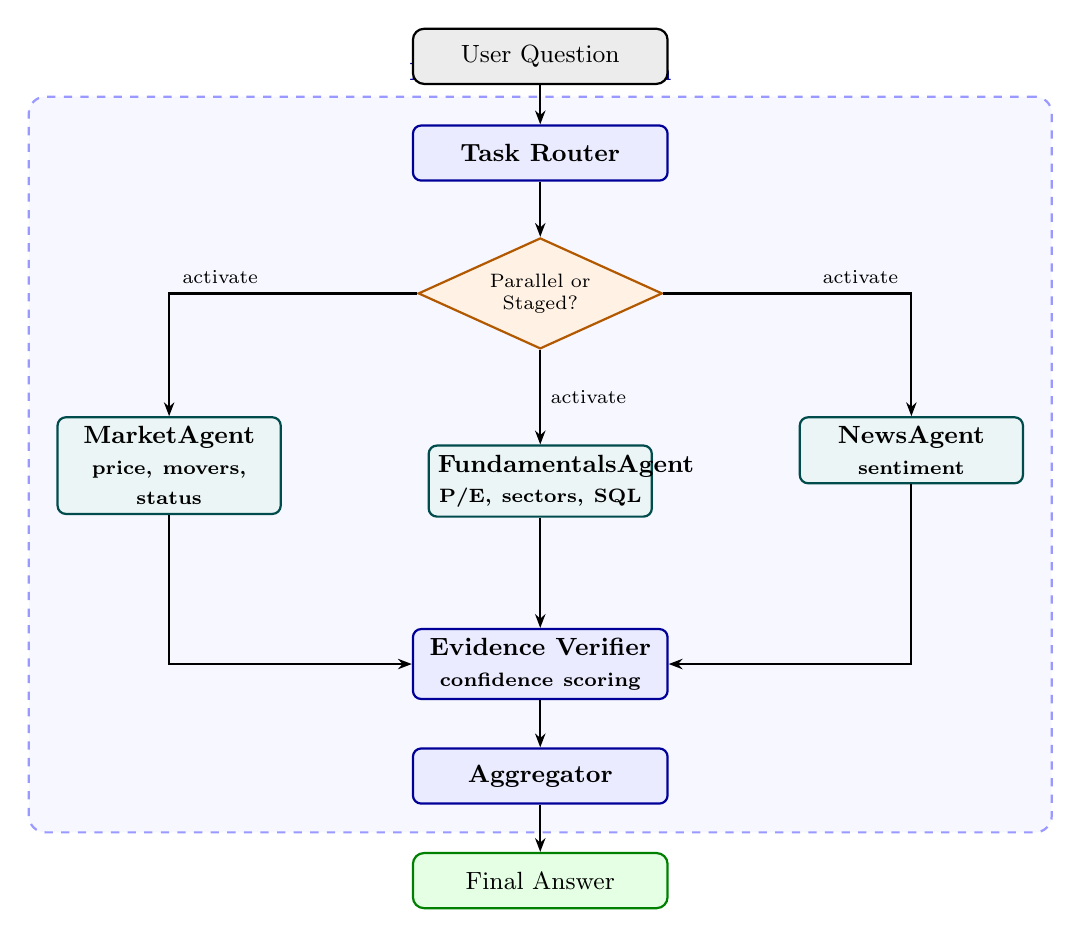
\begin{tikzpicture}[node distance=0.5cm and 1.8cm]

  % ---- Nodes ----
  \node[io]       (user)   {User Question};

  \node[agent, below=of user]    (router)  {Task Router};

  \node[decision, below=0.7cm of router](mode) {Parallel or\\Staged?};

  % Specialists (parallel row)
  \node[specialist, below left=1.2cm and 2.5cm of mode]  (market) {MarketAgent\\{\scriptsize price, movers, status}};
  \node[specialist, below=1.2cm of mode]                 (fund)   {FundamentalsAgent\\{\scriptsize P/E, sectors, SQL}};
  \node[specialist, below right=1.2cm and 2.5cm of mode] (news)   {NewsAgent\\{\scriptsize sentiment}};

  % Verifier
  \node[agent, below=1.4cm of fund]  (verifier) {Evidence Verifier\\{\scriptsize confidence scoring}};

  % Aggregator
  \node[agent, below=0.6cm of verifier] (agg)  {Aggregator};

  \node[answer, below=0.6cm of agg]    (resp) {Final Answer};

  % ---- Arrows ----
  \draw[arr] (user)   -- (router);
  \draw[arr] (router) -- (mode);

  \draw[arr] (mode) -| node[lbl, above left, pos=0.3]{activate} (market);
  \draw[arr] (mode) --  node[lbl, right]{activate} (fund);
  \draw[arr] (mode) -| node[lbl, above right, pos=0.3]{activate} (news);

  \draw[arr] (market)  |- (verifier);
  \draw[arr] (fund)    -- (verifier);
  \draw[arr] (news)    |- (verifier);

  \draw[arr] (verifier) -- (agg);
  \draw[arr] (agg)      -- (resp);

  % ---- Bounding boxes ----
  \begin{scope}[on background layer]
    \node[draw=blue!40, fill=blue!3, thick, dashed, rounded corners=6pt,
          fit=(router)(mode)(market)(fund)(news)(verifier)(agg),
          inner sep=10pt,
          label={[blue!60!black, font=\small\bfseries]above:Multi-Agent System}]
          {};
  \end{scope}

\end{tikzpicture}
\caption{Design diagram of the Adaptive Router-Verifier multi-agent architecture.
The Task Router selects which specialist agents to activate and whether to run them
in parallel or staged mode.  Each specialist's output is scored by the Evidence Verifier
before the Aggregator merges findings into a single answer.}
\label{fig:design}
\end{figure*}

% -----------------------------------------------------------------------
\section{Implementation Details}
% -----------------------------------------------------------------------

\subsection{Technology Stack}
\begin{itemize}
  \item \textbf{OpenAI API} (\texttt{gpt-4o-mini}, \texttt{gpt-4o}) -- all LLM calls
        and tool-calling via the function-calling API.
  \item \textbf{Alpha~Vantage} (premium key) -- market status, top movers, news sentiment,
        and company fundamentals.
  \item \textbf{yfinance} -- price performance data and fundamentals fallback.
  \item \textbf{SQLite} (\texttt{stocks.db}) -- local database of S\&P~500 companies
        with sector, industry, market cap, and exchange.
  \item \textbf{Streamlit} -- web interface with session-state conversational memory.
  \item \textbf{python-dotenv} -- API keys loaded from \texttt{.env}.
\end{itemize}

\subsection{Agentic Loop}

All agents share a single \texttt{run\_specialist\_agent()} function that implements
the core loop: send the system prompt and task to the LLM, execute any tool calls,
append tool results to the conversation, and repeat until the model produces a final
text response or the iteration limit (8) is reached.  Tool dispatch uses a name-to-function
dictionary, and all tool results are serialised as JSON.

\subsection{Multi-Agent Execution Modes}

The router's \texttt{execution\_mode} field controls specialist scheduling:
\begin{itemize}
  \item \textbf{Parallel}: all active specialists run concurrently via
        \texttt{ThreadPoolExecutor}.  Used when sub-tasks are independent (most cases).
  \item \textbf{Staged}: the \texttt{staged\_first} agent runs first, and its answer
        is appended as context to the remaining agents' tasks before they run in parallel.
        Used for dependency chains like ``find tickers, then get their performance.''
\end{itemize}

\subsection{Conversational Memory (Streamlit)}

The Streamlit app maintains a \texttt{st.session\_state["messages"]} list of all
user/assistant turns.  Before each agent call, the \texttt{build\_question\_with\_history()}
function prepends the last 6 messages (3 exchanges) to the current question, enabling
agents to resolve follow-up references like ``that,'' ``the two,'' or ``it.''
Long assistant responses are truncated to 800 characters to avoid token bloat.

% -----------------------------------------------------------------------
\section{LLM-as-a-Judge Evaluator}
% -----------------------------------------------------------------------

\subsection{Scoring Rubric}

The evaluator scores each agent answer on a 0--3 scale:
\begin{itemize}
  \item \textbf{3} -- Fully correct: satisfies the expected answer description with no
        invented entities.
  \item \textbf{2} -- Mostly correct: minor omission or slight inaccuracy.
  \item \textbf{1} -- Partially correct: relevant attempt but missing key parts.
  \item \textbf{0} -- Incorrect or refusal.
\end{itemize}

\subsection{Hallucination Detection}

A critical design challenge: the evaluator must distinguish between tool-retrieved precise
values (legitimate) and training-data guesses presented as facts (hallucinations).
Our evaluator uses two layers:

\paragraph{Rule-based pre-check}
If the expected answer requires tool retrieval (contains phrases like ``from Alpha Vantage'')
\emph{and} the agent's answer uses hedging language (``approximately,'' ``based on current
market conditions,'' ``around''), the answer is immediately flagged as a hallucination
with score~1.  Refusals are \emph{not} flagged as hallucinations.

\paragraph{LLM judge}
For all other cases, the evaluator prompts the LLM with a detailed rubric including
worked examples for tool-retrieved values (not hallucination), hedged estimates
(hallucination), and refusals (not hallucination, score~0).

\subsection{Calibration}

Three calibration tests verify correct behaviour:
(1)~a precise P/E value scores~3 with no hallucination detected,
(2)~an ``approximately'' estimate is flagged as hallucination with score~$\leq$1, and
(3)~a refusal scores~0 with no hallucination.

% -----------------------------------------------------------------------
\section{Results}
% -----------------------------------------------------------------------

\subsection{Overall Performance (gpt-4o-mini)}

Table~\ref{tab:mini} reports the per-tier and overall accuracy from
\texttt{results\_gpt4o\_mini.xlsx}.

\begin{table}[H]
\centering
\caption{Evaluation results by architecture and difficulty tier (gpt-4o-mini).}
\label{tab:mini}
\begin{tabular}{lcccc}
\toprule
\textbf{Architecture} & \textbf{Easy} & \textbf{Medium} & \textbf{Hard} & \textbf{Overall} \\
\midrule
Baseline      & 26.7\% & 0\%    & 0\%    & 11.1\% \\
Single Agent  & 80.0\% & 86.7\% & 33.3\% & 75.0\% \\
Multi-Agent   & 93.3\% & 86.7\% & 50.0\% & 83.3\% \\
\bottomrule
\end{tabular}
\end{table}

\subsection{Overall Performance (gpt-4o)}

Table~\ref{tab:large} reports the same metrics with \texttt{gpt-4o}.

\begin{table}[H]
\centering
\caption{Evaluation results by architecture and difficulty tier (gpt-4o).}
\label{tab:large}
\begin{tabular}{lcccc}
\toprule
\textbf{Architecture} & \textbf{Easy} & \textbf{Medium} & \textbf{Hard} & \textbf{Overall} \\
\midrule
Baseline      & 26.7\% & 0\%    & 0\%    & 8.9\% \\
Single Agent  & 73.3\% & 86.7\% & 40.0\% & 66.7\% \\
Multi-Agent   & 80.0\% & 80.0\% & 40.0\% & 66.7\% \\
\bottomrule
\end{tabular}
\end{table}

\subsection{Baseline vs.\ Single Agent}

The baseline scored 11.1\% overall (gpt-4o-mini) because it has no access to live data.
On easy questions like Q01 (list semiconductor companies), the baseline earned partial
credit by recalling well-known tickers from training data, but on any question requiring
a current number (Q03: AAPL P/E ratio, Q05: NVDA 1-month performance), it either refused
or guessed.  The single agent's 75\% accuracy is entirely attributable to tool access:
it retrieves live data before answering, eliminating the fundamental information gap.

\subsection{Single Agent vs.\ Multi-Agent}

With gpt-4o-mini, Multi-Agent (83.3\%) outperformed Single Agent (75\%) overall,
with the largest gap on easy questions (93.3\% vs.\ 80\%) and hard questions
(50\% vs.\ 33.3\%).  On easy questions the improvement comes from cleaner tool usage:
the router activates only the relevant specialist, reducing the chance of the model
calling an unnecessary tool or getting confused by schema options.  On hard questions
like Q13 (top 3 semiconductor stocks by return + P/E + sentiment), the specialist
decomposition allows each agent to focus on its domain rather than juggling 8+ tool
calls in a single context window.

However, Multi-Agent also introduces overhead.  On medium questions like Q06 (compare
1-year returns for 3 tickers), Single Agent solves the problem with one
\texttt{get\_price\_performance} call.  The Multi-Agent system routes it through an
orchestrator, spins up a MarketAgent, then runs an aggregator -- producing the same
answer with 2--3$\times$ the latency.

\subsection{gpt-4o-mini vs.\ gpt-4o}

Surprisingly, gpt-4o did not consistently outperform gpt-4o-mini.  For the Multi-Agent
architecture, gpt-4o-mini achieved 83.3\% overall vs.\ gpt-4o's 66.7\%.  The larger model
was more conservative: on Q11 (tech stocks that dropped this month but grew this year),
gpt-4o's Multi-Agent concluded ``no verified stocks meet the criteria'' rather than
returning partial results, while gpt-4o-mini at least identified one qualifying stock.
The larger model also had more hallucination flags (3 vs.\ 2 for Multi-Agent), primarily
on Q10 and Q14 where the evaluator flagged values it could not confirm as tool-retrieved.

On easy and medium single-domain questions, both models performed comparably, suggesting
that the smaller model is sufficient for straightforward tool-calling tasks and the
cost of gpt-4o is not justified for this workload.

\subsection{Hallucination Analysis}

The baseline produced zero hallucinations because it consistently refused rather than
guessing -- the safest failure mode.  The Single Agent had 1 hallucination flag
(gpt-4o-mini) on Q10 where Goldman Sachs' 52-week values appeared implausible.
The Multi-Agent system had 2 hallucinations (gpt-4o-mini), both on fundamentals
questions where the aggregator reported values without sufficient evidence of tool
retrieval.  With gpt-4o, hallucinations increased to 3, partly due to the evaluator's
stricter assessment of the larger model's outputs.

\subsection{Latency}

Average response times reflect the architectural complexity:
Baseline~$\approx$2.6s, Single Agent~$\approx$5.3s, Multi-Agent~$\approx$10.2s
(gpt-4o-mini).  The Multi-Agent overhead is acceptable for complex cross-domain
questions where it adds value, but represents unnecessary cost for simple queries.

% -----------------------------------------------------------------------
\section{Challenges and Design Decisions}
% -----------------------------------------------------------------------

\paragraph{Router accuracy}
The Task Router occasionally misclassifies domain requirements.  For Q15 (finance sector
stocks near 52-week low + sentiment), the router correctly identified all three domains
but the FundamentalsAgent failed to retrieve finance sector tickers because it searched
for ``Finance'' instead of ``Financials'' (the actual sector name in the database).
This cascading failure caused the entire pipeline to return no data.

\paragraph{Staged vs.\ parallel execution}
Many hard questions have implicit dependencies: ``find the top 3 stocks by X, then get
Y for each.''  The router must detect these dependencies and use staged execution so
that the first agent's output (the ticker list) is available to subsequent agents.
When the router incorrectly chooses parallel mode, the downstream agents lack the
tickers they need and either guess or fail.

\paragraph{Evidence Verifier limitations}
The rule-based verifier scores confidence mechanically based on tool usage and answer
length.  It cannot detect \emph{semantic} errors -- for example, an agent that calls
the correct tool but misinterprets the result.  A more sophisticated verifier could
cross-check the agent's textual claims against the raw tool output JSON, but this would
require an additional LLM call per specialist.

\paragraph{Alpha~Vantage rate limiting}
The premium API key mitigates most rate limits, but concurrent specialist calls in
parallel mode can still trigger throttling.  Tool~6 (\texttt{get\_company\_overview})
includes a \texttt{yfinance} fallback to handle this gracefully.

\paragraph{Evaluator bias}
The LLM-as-a-Judge tends toward leniency: it sometimes awards a score of~2 to answers
that are substantively incomplete.  The rule-based pre-check for hedging language helps
catch the most egregious cases, but the evaluator still struggles with partial answers
that look plausible but omit critical data points.

% -----------------------------------------------------------------------
\section{Streamlit Deployment}
% -----------------------------------------------------------------------

The Streamlit app (\texttt{streamlitapp/app.py}) wraps the notebook agents into a
chat interface with:

\begin{itemize}
  \item \textbf{Sidebar controls}: Agent selector (Single Agent / Multi-Agent) and
        model selector (gpt-4o-mini / gpt-4o).
  \item \textbf{Conversation history}: full display of user and assistant messages,
        with metadata captions showing architecture, model, tools called, elapsed time,
        and average confidence.
  \item \textbf{Conversational memory}: the last 6 messages are prepended to each new
        question, enabling 3-turn follow-up resolution.
  \item \textbf{Clear conversation}: resets \texttt{st.session\_state} and reruns the app.
\end{itemize}

The app imports directly from \texttt{agents.py}, which mirrors the notebook code with
adjustments for absolute paths (resolved via \texttt{\_\_file\_\_}), explicit
\texttt{model} parameters (no global \texttt{ACTIVE\_MODEL}), and \texttt{verbose=False}
defaults for clean Streamlit output.

% -----------------------------------------------------------------------
\section{Head-to-Head: Two Multi-Agent Architectures}
% -----------------------------------------------------------------------

To understand how architectural choices affect performance independent of the benchmark
design, we ran a head-to-head comparison of the two team members' multi-agent
implementations on the same 15 questions using \texttt{gpt-4o-mini}, cross-evaluated by
both team members' LLM-as-a-Judge evaluators.

\subsection{Architectural Differences}

Table~\ref{tab:arch-diff} summarises the key design differences.

\begin{table}[H]
\centering
\caption{Architectural comparison of the two multi-agent systems.}
\label{tab:arch-diff}
\begin{tabular}{p{2.2cm}p{2.8cm}p{2.8cm}}
\toprule
\textbf{Component} & \textbf{Eugenio (Adaptive Router-Verifier)} & \textbf{Oguz (Orchestrator-Critic)} \\
\midrule
Router output & domain flags + execution mode & agent list + phased flag + per-agent sub-tasks \\
Specialists   & MarketAgent, FundamentalsAgent, NewsAgent & Price Agent, Fundamentals Agent, Sentiment Agent \\
Verification  & Rule-based confidence scoring (no LLM) & LLM Critic checks answer vs.\ raw tool data \\
Synthesis     & LLM Aggregator merges by confidence rank & LLM Synthesizer with TABLE/PROSE format rules \\
Specialist prompts & Concise, 2--3 sentence role descriptions & Detailed protocols (scratchpad for ranking, multi-condition filtering) \\
\bottomrule
\end{tabular}
\end{table}

The most significant design differences are: (1)~Oguz's specialist prompts include
explicit step-by-step protocols for ranking and filtering, while Eugenio's rely on the
model's general instruction-following; (2)~Oguz uses an LLM-based Critic that validates
each specialist's answer against its raw tool output, while Eugenio uses a cheaper
rule-based verifier; and (3)~Oguz's orchestrator writes focused sub-tasks per agent,
while Eugenio's router only flags which domains are needed.

\subsection{Evaluator Differences}

Eugenio's evaluator uses a two-layer approach: a deterministic pre-check flags hedging
language as hallucination (score~1) before the LLM judge runs, reducing false negatives
on the most common fabrication pattern.  Oguz's evaluator is purely LLM-based but
includes domain-specific guidance: precise decimals are treated as evidence of real tool
calls even when paired with ``approximately,'' and live data values are never compared
against training knowledge.

\subsection{Head-to-Head Results}

Table~\ref{tab:h2h} shows the per-question scores assigned by both evaluators.

\begin{table}[H]
\centering
\caption{Head-to-head comparison (gpt-4o-mini).  Each cell shows the score out of~3
assigned by the named evaluator to the named architecture.}
\label{tab:h2h}
\small
\begin{tabular}{llcccc}
\toprule
 & & \multicolumn{2}{c}{\textbf{Eugenio MA}} & \multicolumn{2}{c}{\textbf{Oguz MA}} \\
\cmidrule(lr){3-4} \cmidrule(lr){5-6}
\textbf{QID} & \textbf{Tier} & \textbf{E-eval} & \textbf{O-eval} & \textbf{E-eval} & \textbf{O-eval} \\
\midrule
Q01 & easy   & 2 & 3 & 2 & 3 \\
Q02 & easy   & 2 & 2 & 2 & 2 \\
Q03 & easy   & 3 & 3 & 3 & 3 \\
Q04 & easy   & 1 & 1 & 1 & 1 \\
Q05 & easy   & 3 & 3 & 0 & 0 \\
Q06 & medium & 3 & 3 & 2 & 2 \\
Q07 & medium & 3 & 3 & 3 & 3 \\
Q08 & medium & 2 & 2 & 2 & 2 \\
Q09 & medium & 3 & 2 & 2 & 1 \\
Q10 & medium & 2 & 1 & 2 & 1 \\
Q11 & hard   & 1 & 1 & 2 & 1 \\
Q12 & hard   & 1 & 0 & 3 & 3 \\
Q13 & hard   & 2 & 2 & 2 & 2 \\
Q14 & hard   & 3 & 3 & 2 & 2 \\
Q15 & hard   & 0 & 0 & 0 & 0 \\
\bottomrule
\end{tabular}
\end{table}

\subsection{Analysis}

\paragraph{Overall scores}
Averaging across both evaluators, Eugenio's architecture scored 2.00/3 (66.7\% accuracy)
and Oguz's scored 1.80/3 (60.0\%).  On a per-question basis, Eugenio won 4 questions,
Oguz won 2, and 9 were ties.  Both systems failed completely on Q15 (finance sector
stocks near 52-week low), which requires chaining sector lookup, fundamentals retrieval,
proximity computation, and sentiment -- the most complex question in the benchmark.

\paragraph{Easy tier}
Eugenio's system averaged 2.30/3 vs.\ Oguz's 1.70/3.  The gap is driven almost entirely
by Q05 (NVDA 1-month performance): Oguz's synthesizer dropped the start and end prices
from the final answer, reporting only the percentage change, which both evaluators scored
as~0 for missing required fields.  This highlights a weakness of strict output format
rules -- the TABLE/PROSE format in Oguz's synthesizer optimised for certain question
patterns but penalised others.

\paragraph{Hard tier}
Oguz's system performed better on Q12 (large-cap NASDAQ tech stocks $>$20\% YTD), scoring
3/3 vs.\ Eugenio's 0.5/3.  Oguz's detailed Price Agent prompt includes an explicit
multi-condition filtering protocol that correctly handled the dual filter (market cap +
exchange + YTD threshold).  Eugenio's MarketAgent lacked this protocol and returned
incorrect results.  Conversely, Eugenio won Q14 (compare JPM, GS, BAC across 3 metrics)
because the Adaptive Router correctly activated both MarketAgent and FundamentalsAgent
in parallel, while Oguz's system produced a less complete synthesis.

\paragraph{Prompt engineering matters more than architecture}
The largest quality differences were driven not by the pipeline structure (both use
router $\to$ specialists $\to$ verification $\to$ synthesis) but by prompt specificity.
Oguz's Price Agent prompt with its ``scratchpad protocol'' and ``multi-condition filtering
protocol'' produced measurably better results on ranking and filtering questions.
Eugenio's simpler prompts worked well on straightforward queries but degraded on
questions requiring precise multi-step reasoning within a single specialist.

\paragraph{Verification trade-offs}
Eugenio's rule-based verifier is fast (no LLM call) but shallow -- it checks \emph{whether}
tools were called, not \emph{whether the answer matches the tool output}.  Oguz's LLM
Critic cross-checks the answer against raw tool data, catching cases where a specialist
calls the right tool but misreports the result.  However, the Critic adds latency:
Oguz's system averaged 25.6s per question vs.\ Eugenio's 8.8s, with Q15 taking 250s
due to the Critic evaluating large volumes of fundamentals data for many finance tickers.

\paragraph{Evaluator agreement}
The two evaluators agreed on the exact score for 73\% of answer evaluations (22/30).
When they disagreed, Eugenio's evaluator tended to be slightly more generous (awarding
score~2 where Oguz's gave~1), likely because Eugenio's rule-based pre-check only catches
hedging-based hallucinations while Oguz's LLM evaluator also penalises incomplete answers
more aggressively.

\paragraph{Latency}
Eugenio's system was 2.9$\times$ faster on average (8.8s vs.\ 25.6s).  The primary
driver is the verification stage: Eugenio's rule-based verifier adds negligible time,
while Oguz's LLM Critic requires one additional API call per specialist.  On Q15, Oguz's
system took over 4 minutes because the Fundamentals Agent fetched overview data for
dozens of finance-sector tickers, and the Critic then had to process all that raw data.

% -----------------------------------------------------------------------
\section{Conclusion}
% -----------------------------------------------------------------------

The project demonstrates that tool access is the single most important factor for
financial Q\&A: the baseline's 11\% accuracy vs.\ the single agent's 75\% is entirely
explained by the ability to retrieve live data.  The multi-agent architecture provides
a further 8-point improvement (83\% overall with gpt-4o-mini) by decomposing complex
cross-domain questions into specialist sub-tasks with evidence verification, though it
adds latency and offers no benefit on simple single-domain queries.

The head-to-head comparison of two independently developed multi-agent systems reveals
that \textbf{prompt engineering within specialists matters more than pipeline structure}.
Both systems use the same high-level pattern (router $\to$ specialists $\to$ verification
$\to$ synthesis), yet per-question results diverge significantly based on how detailed
the specialist prompts are.  Oguz's explicit ranking and filtering protocols improved
hard-question accuracy, while Eugenio's simpler prompts and rule-based verifier delivered
comparable results 3$\times$ faster.  The evaluator comparison showed 73\% agreement,
with systematic differences in how each handles partial answers -- confirming that
LLM-as-a-Judge reliability remains an open challenge for automated evaluation.

Surprisingly, the larger gpt-4o model did not outperform gpt-4o-mini in our evaluation,
suggesting that for structured tool-calling tasks, the smaller model is cost-effective.
The primary architectural weakness shared by both systems is the router's dependency
detection: when it fails to recognise a staged execution requirement, specialists lack
the context they need, causing cascading failures on hard questions.

\end{document}
